\documentclass[10pt,a4paper]{article}
    \usepackage[a4paper, total={6.5in, 8in}, textheight = 700pt]{geometry}
    \usepackage[utf8]{inputenc}
    \usepackage{fancyhdr}
    \usepackage{listings}
    % \usepackage{minted}
    \usepackage{amsmath}
    \usepackage{amsfonts}
    \usepackage{amssymb}
    \usepackage{graphicx}
    \usepackage{wrapfig}
    \usepackage{caption}
    \usepackage{subcaption}
    \usepackage{float}
    \usepackage[space]{grffile}
    \usepackage{hyperref}
    \usepackage{multirow}
    \usepackage{booktabs}
    \usepackage{amsmath}
    \usepackage{multicol}
    \usepackage{enumitem}
    \usepackage{pageslts}
    \usepackage{setspace}
    \usepackage{color}
    \usepackage{xcolor}
    \usepackage{array}
    \usepackage{enumitem}
    \usepackage{libertine}
    \usepackage{lscape}
    \usepackage{pdfpages}
    \usepackage{pdflscape}
    \usepackage{tcolorbox}
    %% \usepackage[switch, modulo]{lineno}
    
    \definecolor{dkgreen}{rgb}{0,0.6,0}
    \definecolor{gray}{rgb}{0.5,0.5,0.5}
    \definecolor{mauve}{rgb}{0.58,0,0.82}
    \definecolor{yellowq}{RGB}{250,200,45}
    \definecolor{lightgray}{rgb}{0.95, 0.95, 0.95}
    \definecolor{darkgray}{rgb}{0.4, 0.4, 0.4}
    %\definecolor{purple}{rgb}{0.65, 0.12, 0.82}
    \definecolor{editorGray}{rgb}{0.95, 0.95, 0.95}
    \definecolor{editorOcher}{rgb}{1, 0.5, 0} % #FF7F00 -> rgb(239, 169, 0)
    \definecolor{editorGreen}{rgb}{0, 0.5, 0} % #007C00 -> rgb(0, 124, 0)
    \definecolor{orange}{rgb}{1,0.45,0.13}		
    \definecolor{olive}{rgb}{0.17,0.59,0.20}
    \definecolor{brown}{rgb}{0.69,0.31,0.31}
    \definecolor{purple}{rgb}{0.38,0.18,0.81}
    \definecolor{lightblue}{rgb}{0.1,0.57,0.7}
    \definecolor{lightred}{rgb}{1,0.4,0.5}
    
    \newcommand{\musthave}{\colorbox{red}{Must-have}}
    \newcommand{\shouldhave}{\colorbox{yellowq}{Should-have}}
    \newcommand{\couldhave}{\colorbox{dkgreen}{Could-have}}
    \newcommand{\wouldhave}{\colorbox{cyan}{Would-have}}
    
    \lstset{frame=tb,
      language=Java,
      aboveskip=1.5mm,
      belowskip=1.5mm,
      showstringspaces=false,
      columns=flexible,
      numbers=left,
      numberstyle=\tiny\color{gray},
      keywordstyle=\color{blue},
      commentstyle=\color{dkgreen},
      stringstyle=\color{mauve},
      breaklines=true,
      breakatwhitespace=true,
      tabsize=3,
      texcl = true
    }   
    
    % CSS
    \lstdefinelanguage{CSS}{
      keywords={color,background-image:,margin,padding,font,weight,display,position,top,left,right,bottom,list,style,border,size,white,space,min,width, transition:, transform:, transition-property, transition-duration, transition-timing-function},	
      sensitive=true,
      morecomment=[l]{//},
      morecomment=[s]{/*}{*/},
      morestring=[b]',
      morestring=[b]",
      alsoletter={:},
      alsodigit={-}
    }
    
    % JavaScript
    \lstdefinelanguage{JavaScript}{
      morekeywords={typeof, new, true, false, catch, function, return, null, catch, switch, var, if, in, while, do, else, case, break},
      morecomment=[s]{/*}{*/},
      morecomment=[l]//,
      morestring=[b]",
      morestring=[b]'
    }
    
    \lstdefinelanguage{HTML5}{
      language=html,
      sensitive=true,	
      alsoletter={<>=-},	
      morecomment=[s]{<!-}{-->},
      tag=[s],
      otherkeywords={
      % General
      >,
      % Standard tags
        <!DOCTYPE,
      </html, <html, <head, <title, </title, <style, </style, <link, </head, <meta, />,
        % body
        </body, <body,
        % Divs
        </div, <div, </div>, 
        % Paragraphs
        </p, <p, </p>,
        % scripts
        </script, <script,
      % More tags...
      <canvas, /canvas>, <svg, <rect, <animateTransform, </rect>, </svg>, <video, <source, <iframe, </iframe>, </video>, <image, </image>, <header, </header, <article, </article
      },
      ndkeywords={
      % General
      =,
      % HTML attributes
      charset=, src=, id=, width=, height=, style=, type=, rel=, href=,
      % SVG attributes
      fill=, attributeName=, begin=, dur=, from=, to=, poster=, controls=, x=, y=, repeatCount=, xlink:href=,
      % properties
      margin:, padding:, background-image:, border:, top:, left:, position:, width:, height:, margin-top:, margin-bottom:, font-size:, line-height:,
        % CSS3 properties
      transform:, -moz-transform:, -webkit-transform:,
      animation:, -webkit-animation:,
      transition:,  transition-duration:, transition-property:, transition-timing-function:,
      }
    }
    
    \lstdefinestyle{htmlcssjs} {%
      % General design
    %  backgroundcolor=\color{editorGray},
      basicstyle={\footnotesize\ttfamily},   
      frame=b,
      % line-numbers
      xleftmargin={0.75cm},
      numbers=left,
      stepnumber=1,
      firstnumber=1,
      numberfirstline=true,	
      % Code design
      identifierstyle=\color{black},
      keywordstyle=\color{blue}\bfseries,
      ndkeywordstyle=\color{editorGreen}\bfseries,
      stringstyle=\color{editorOcher}\ttfamily,
      commentstyle=\color{brown}\ttfamily,
      % Code
      language=HTML5,
      alsolanguage=JavaScript,
      alsodigit={.:;},	
      tabsize=2,
      showtabs=false,
      showspaces=false,
      showstringspaces=false,
      extendedchars=true,
      breaklines=true,
      % German umlauts
      literate=%
      {Ö}{{\"O}}1
      {Ä}{{\"A}}1
      {Ü}{{\"U}}1
      {ß}{{\ss}}1
      {ü}{{\"u}}1
      {ä}{{\"a}}1
      {ö}{{\"o}}1
    }
    
    
    %%%%%%%%%%%%% PAGE LAYOUT %%%%%%%%%%%%%
    %\setstretch{1.25}
    %\textwidth=16.5cm
    %\textheight=24cm
    %\voffset=-60pt
    %\hoffset=-60pt
    \setlength{\parindent}{0cm} %No indentation in new paragraph
    \newcommand{\HRule}{\rule{\linewidth}{0.5mm}}
    \pagestyle{fancy}
    \fancyhf{} 
    %%%%%%%%%%%%% PAGE LAYOUT %%%%%%%%%%%%%
    
    
    %%%%%%%%%%%%% HEADER / FOOTER %%%%%%%%%%%%%
    \lhead{Gruppe 13} % Skriv gruppe nummer/navn her
    \chead{CDIO-Final} % Titel på projektet
    \rhead{Juni 2018} % Afleverings måned
    %%%%%%%%%%%%% HEADER / FOOTER %%%%%%%%%%%%%
    
    
    %%%%%%%%%%%%% TABLE LAYOUT OPTIONS %%%%%%%%%%%%%
    \newcolumntype{L}[1]{>{\raggedright\let\newline\\\arraybackslash\hspace{0pt}}m{#1}}
    \newcolumntype{C}[1]{>{\centering\let\newline\\\arraybackslash\hspace{0pt}}m{#1}}
    \newcolumntype{R}[1]{>{\raggedleft\let\newline\\\arraybackslash\hspace{0pt}}m{#1}}
    %%%%%%%%%%%%% TABLE LAYOUT OPTIONS %%%%%%%%%%%%%
    
    
    %%%%%%%%%%%%% LIST LAYOUT 1 %%%%%%%%%%%%%
    \setlistdepth{9}
    
    \newlist{myEnumerate}{enumerate}{9}
    \setlist[myEnumerate,1]{label=(\arabic*)}
    \setlist[myEnumerate,2]{label=(\Roman*)}
    \setlist[myEnumerate,3]{label=(\Alph*)}
    \setlist[myEnumerate,4]{label=(\roman*)}
    \setlist[myEnumerate,5]{label=(\alph*)}
    \setlist[myEnumerate,6]{label=(\arabic*)}
    \setlist[myEnumerate,7]{label=(\Roman*)}
    \setlist[myEnumerate,8]{label=(\Alph*)}
    \setlist[myEnumerate,9]{label=(\roman*)}
    %%%%%%%%%%%%% LIST LAYOUT 1 %%%%%%%%%%%%%
    %%%%%%%%%%%%% LIST LAYOUT 2 %%%%%%%%%%%%%
    \setlistdepth{9}
    
    \newlist{byEnumerate}{enumerate}{9}
    \setlist[byEnumerate,1]{label= 2\alph*:}
    \setlist[byEnumerate,2]{label=(\alph*)}
    \setlist[byEnumerate,3]{label=(\Alph*)}
    \setlist[byEnumerate,4]{label=(\roman*)}
    \setlist[byEnumerate,5]{label=(\alph*)}
    \setlist[byEnumerate,6]{label=(\arabic*)}
    \setlist[byEnumerate,7]{label=(\Roman*)}
    \setlist[byEnumerate,8]{label=(\Alph*)}
    \setlist[byEnumerate,9]{label=(\roman*)}
    %%%%%%%%%%%%% LIST LAYOUT 2 %%%%%%%%%%%%%
    
    %%%%%%%%%%%%% BEGIN DOCUMENT %%%%%%%%%%%%%
    \begin{document}
    \pagenumbering{arabic}
    \thispagestyle{plain}
    %%%%%%%%%%%%% BEGIN DOCUMENT %%%%%%%%%%%%%
    
    %%%%%%%%%%%%% FRONT PAGE %%%%%%%%%%%%%
    \begin{titlepage}
\begin{center}


\includegraphics{Pictures/frontpage/dtu-logo.png}~\\[0.5cm]
\textsc{\Large Sens MOTION } \\% Kursus navn1

% Title
\HRule 
{ \huge \bfseries CDIO Final \\[0.1cm] } % Titel på projekt

\HRule \\[0.8cm]
\textsc{Gruppe 6}
%%% NEED FIX %%%
\begin{multicols}{5}
\begin{figure}[H]
        \centering
        
\includegraphics[scale=0.8]{Pictures/frontpage/kim.png}\\
        \textsc{Kim Sandberg Bossen}
        
        \textsc{s163290}\\
        \hfill \break
        \hfill \break
    \end{figure}
\columnbreak
    \begin{figure}[H]
        \centering
        
\includegraphics[scale=0.6]{Pictures/frontpage/Thyge.png}\\
        \textsc{Thyge S. Steffensen}
        
        \textsc{s175176}\\
        \hfill \break
        \hfill \break
    \end{figure}
\columnbreak
    \begin{figure}[H]
        \centering
        
\includegraphics[scale=0.8]{Pictures/frontpage/mathias.png}\\
        \textsc{Mathias M. Thejsen}
        
        \textsc{s175192}\\
        \hfill \break
        \hfill \break
    \end{figure}
\columnbreak
    \begin{figure}[H]
        \centering
        
\includegraphics[scale=0.8]{Pictures/frontpage/jeppe.png}\\
        \textsc{Jeppe Trip \\Kofoed}
        
        \textsc{s175197}\\
        \hfill \break
        \hfill \break
    \end{figure}
\columnbreak
    \begin{figure}[H]
        \centering
        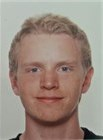
\includegraphics[scale=0.8]{Pictures/frontpage/christian.png}\\
        \textsc{Christian Stahl Andersen}
        
        \textsc{s164150}\\
        \hfill \break
        \hfill \break
    \end{figure}
\end{multicols}
\flushleft
\centering \today % Dags dato
\vfill
\flushleft
\centering \textit{\href{http://207.154.253.254:8080/13\_CDIO\_FINAL/}{http://207.154.253.254:8080/13\_CDIO\_FINAL/}}
\vfill
\end{center}

\end{titlepage}

    %%%%%%%%%%%%% FRONT PAGE %%%%%%%%%%%%%
    
    
    %%%%%%%%%%%%% TABLE OF CONTENT %%%%%%%%%%%%%
    \newpage
    \tableofcontents
    \cleardoublepage
    \cfoot{Page \thepage\ of \lastpageref{LastPage}}
    %%%%%%%%%%%%% TABLE OF CONTENT %%%%%%%%%%%%%
    
    %%%%%%%%%%%%% AFTER TABLE OF CONTENT %%%%%%%%%%%%%
    \setcounter{page}{1}
    \def\emptyline{\vspace{12pt}}
     
    
    \end{document}